\section{要求定義}
ユーザが商品識別システムに求める機能や動作を以下に述べる。以下に要求定義をまとめた図\ref{usecase}を載せる。赤枠で囲っている部分が筆者が担当した。
\ref{usecase}では、ユーザが商品識別システムに対して動作を行った際に、システムがどのような振る舞いをするか記載した。ユーザは通常の買い物のように、カートに商品を出し入れすることができる。このときカート(RaspberryPi)が商品に関するデータを集める。解析システムでは、商品の特定とカゴDBへの操作を行う。この解析システムはサーバで動作する。カゴDBは、カート内にある商品の管理を行う。ここで管理されている情報が、最終的な決済システムで利用される。ユーザがカートを返却すると、決済システムが動作する。決済システムは、顧客の所持金からカート内の商品合計金額を引く処理を行う。

\begin{figure}[htbp]
\centering
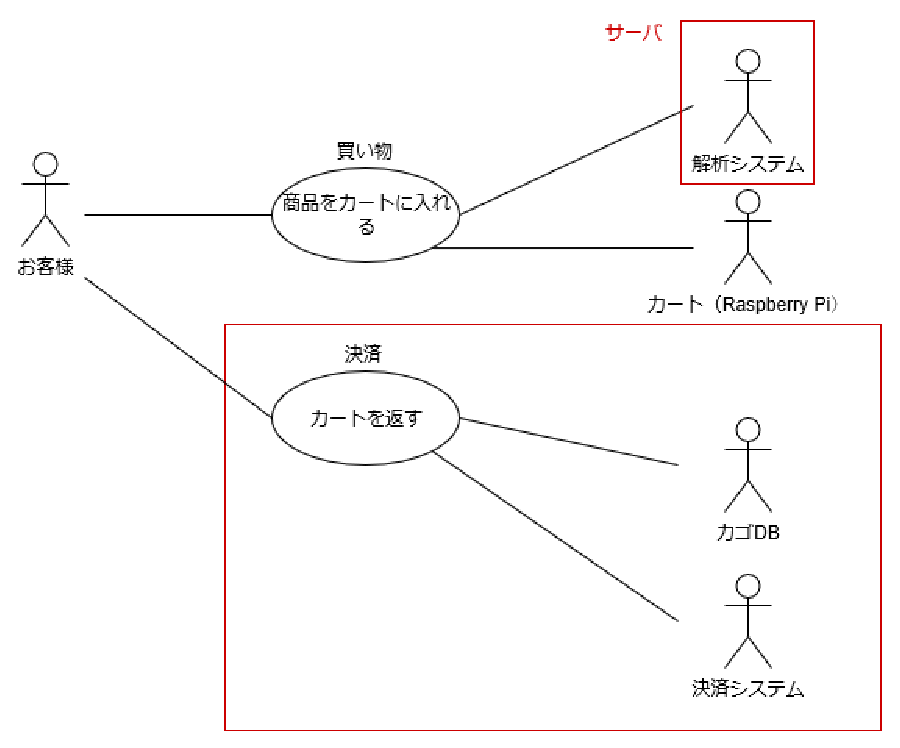
\includegraphics[width=12cm]{./pic/usecase_saishu.eps}
\caption{ユースケース図}
\label{usecase}
\end{figure}